%!TEX root = ../main.tex
%%%%%%%%%%%%%%%%%%%%%%%%%%%%%%%%%%
% Links:
%
% Difficulty:
% Companies: 
%%%%%%%%%%%%%%%%%%%%%%%%%%%%%%%%%%

\chapter{Count the number of islands}
\label{ch:number_islands}

\section{Problem statement}
\begin{exercise}
Write a function that given a $2$D boolean grid of where $1$s represent land and $0$s water counts the number of islands in the grid. An island is surrounded by water and is formed by connecting adjacent lands horizontally or vertically. You may assume all four edges of the grid are all surrounded by water.
The input grid is a 2D \inline{std::vector<std::vector<bool>>} of size $n\times m$. 

	\begin{example}
		\hfill \\
		Given the input grid depicted in Figure \ref{fig:number_islands:example1} the function return $4$.
	The text representation of this example is given below (a $1$ represents land, and a $0$ water):	
	\begin{verbatim}
	1110000
	0100000
	0110110
	0010110
	0100000
	0110010
	0011000
	\end{verbatim}
	\end{example}

\end{exercise}

\begin{figure}
	\centering
	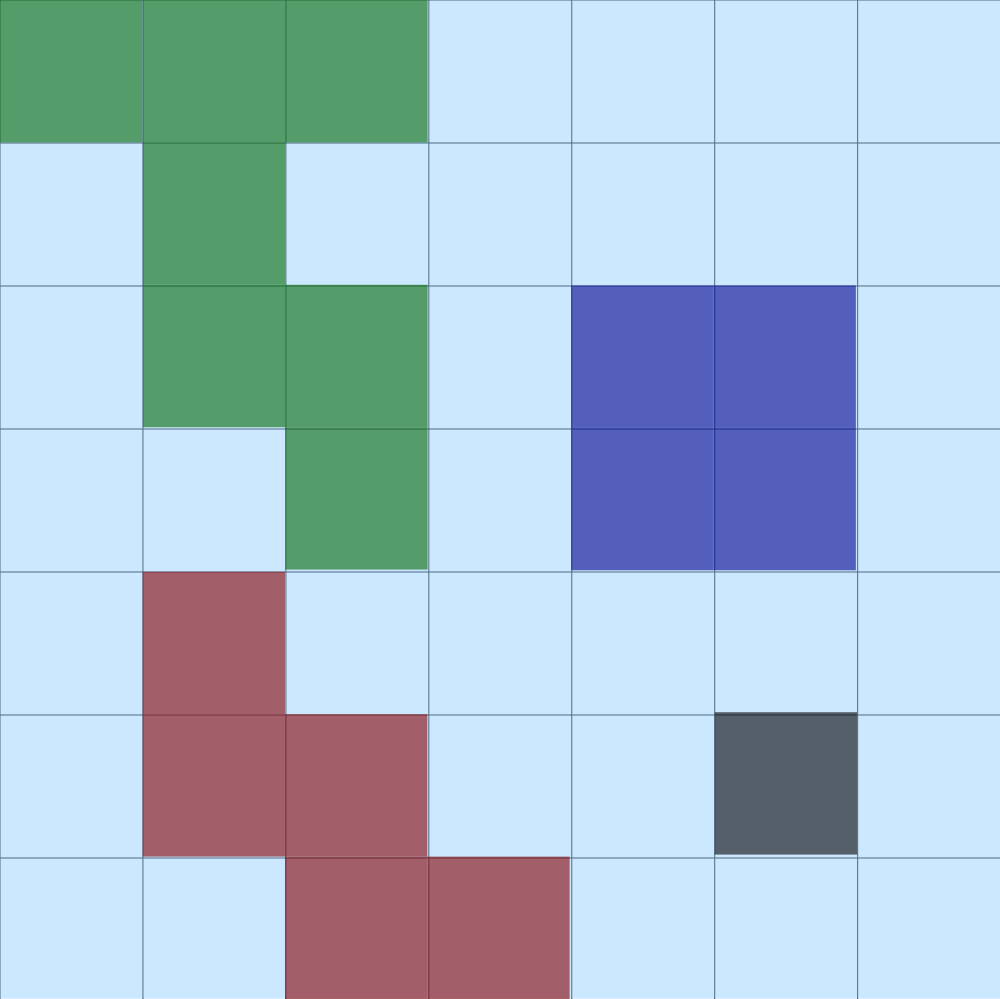
\includegraphics[scale=0.4]{sources/number_islands/images/example1}
	\caption{Visual representation of the example 1 for the problem of counting the number of islands in a map. Cells belonging to the same island share the same color.}
	\label{fig:number_islands:example1}
\end{figure}

\section{Clarification Questions}

\begin{QandA}
	\item Can $n$ or $m$ be $0$?
	\begin{answered}
		\textit{Yes, the map can be empty}
	\end{answered}
	\item Can the input grid be modified?
	\begin{answered}
		\textit{Yes}
	\end{answered}
\end{QandA}

\section{Discussion}
\label{number_islands:sec:discussion}
The problem is asking us to identify portions that are clusters of $1$s. One way to solve it is by looping thought the map one cell at the time until we find a $1$, let's say at cell $(i,j)$. Because this particular $1$ must be part of an island, then what we can do is to start exploring the island one cell at the time until there is no more land on that particular island to visit. When we visit a piece of land (a.k.a. a $1$) we mark it as "visited" or, in other words, as being part of an island. This will be useful because, when we resume our normal linear scanning of the map, we want to make sure we do not count the visited cells as being the starting point of an uncounted island.

For instance w.r.t. the example in Figure \ref{fig:number_islands:example1} we can start out visit at cell $(0,0)$ which is a  $1$ and it is not visited yet. This means that this particular cell is part of a island that we did not count yet. At this point we can start visiting the cells adjacent to $(0,0)$ i.e. cells: $(0,0), (0,1), (0,2), (1,1), (2,1), (2,2), (3,2)$. When a cell is visited is marked as shown in Figure  \ref{fig:number_islands:visited} by the red cross \textcolor[HTML]{860000}{$\times$}.

\begin{figure}
	\centering
	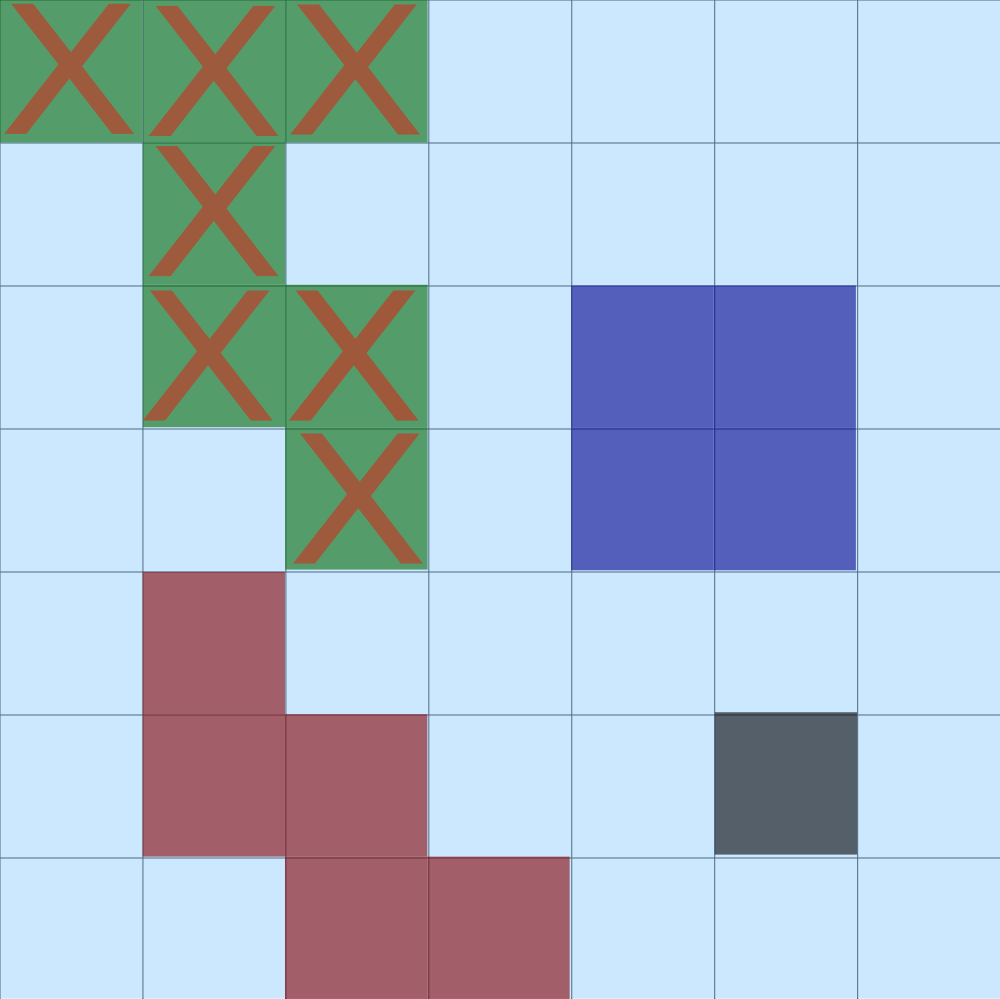
\includegraphics[scale=0.4]{sources/number_islands/images/visited}
	\caption{Visual representation of the example 1 after visiting the cells of the first island.}
	\label{fig:number_islands:example1}
\end{figure}

The visit can be performed using a BFS or DFS approach. In the following section we will shown a recursive and an iterative implementation of the DFS approach. The iterative solution can be turned into a BFS quite easily by just changing the order in which cells are visited.


\subsubsection{DFS iterative}
Listing \ref{list:number_islands:iterative} shows a possible iterative implementation of the DFS approach described above. Note that the core of the algorithm is the function \inline{visit} that uses a stack to keep track of the cells that are still to be visited. For each cell that is actually visited we will also try to visit all piece of yet unvisited land in all four directions (up, down, left and right). We do so by adding them to the pile of cells to be visited. Wen a cell is actually visited, it is marked as so in the variable \inline{visited}.
When we are left with no land left in the stack it means that the island has been completely visited and we can return. 
The function visit returns in the double loop of functions \inline{count_island_iterative_DFS} which will skip all the visited cells and we will trigger another invocation of \inline{visit} as soon as another $1$ is found which has to be part of an unaccounted island.


Also please note how the if at line $22$ takes care of not visiting cells that are outside the boundary of the map, cells that are not land or already visited because this would lead to out-of-bound errors, incorrect results and infinite loops, respectively.

The complexity of this implementation if $O(n\times m)$ for time and space because we will visit the whole map at least once and we will use space proportional to $n\times m$ for the variable \inline{visited}.

\lstinputlisting[language=c++, caption={Iterative DFS solution to the problem of counting the number of islands in a map.},label=list:number_islands:iterative]{sources/number_islands/number_islands_solution1.cpp}

Do we really need to mark the cell as visited by using another different grid? After all, what we need to do is to avoid visiting cells that have been already visited. We can do it by just turning the value in the grid for that cell from land to water and that cell will never be considered part of an island. If we do that, the space complexity does not change because we still use space to store the cells to be visited in the stack, but the amount of space used will be lower in practice. 

\lstinputlisting[language=c++, caption={Alternative iterative DFS solution, without dedicated space for marking visited cells,  to the problem of counting the number of islands in a map.},label=list:number_islands:iterative]{sources/number_islands/number_islands_solution2.cpp}

